\documentclass[11pt]{article}

% ---------------------------------------------------------------------------
%  Wafer-rack equal-Q Navier--Stokes study: audit, correction and verification
% ---------------------------------------------------------------------------
\usepackage[a4paper,margin=1in]{geometry}
\usepackage{amsmath,amssymb}
\usepackage{graphicx}
\usepackage{booktabs}
\usepackage{longtable}
\usepackage{siunitx}
\usepackage{xcolor}
\usepackage{caption}
\usepackage[hidelinks]{hyperref}
\usepackage{float}

\graphicspath{{../figures/}}
\sisetup{round-mode=places,round-precision=5}

\title{\textbf{Wafer-Rack Equal-$Q$ Navier--Stokes Study}\\[2pt]
\large Audit, Correction, and Reproducibility Check}
\author{CFD code review \& reproduction}
\date{\today}

\begin{document}

% ===========================================================================
%  PAGE 1 : TITLE + NOMENCLATURE
% ===========================================================================
\maketitle
\thispagestyle{empty}

\begin{abstract}
A two-dimensional incompressible Navier--Stokes solver for flow through a rack
of six wafers is reviewed, corrected, and re-run. The solver uses
a geometry-aligned Marker-and-Cell (MAC) staggered grid with a fractional-step
(projection) method, first-order donor-cell upwind advection and explicit
second-order diffusion. An equal-rack-flow constraint fixes the inlet velocity
of each pitch by a bracketed scalar root solve. Reproduction reruns
\emph{through the same solver implementation} recover the audited production
inlet speeds and hydraulic resistances, confirm discrete mass conservation at
roundoff ($\sim\!10^{-13}\%$), and recover the ordering
$R_{h,\mathrm{Small}}>R_{h,\mathrm{Medium}}>R_{h,\mathrm{Large}}$. This is a
reproducibility check, not an independent-implementation verification, and grid-
and timestep-independence have not yet been established; the absolute
$U_\mathrm{in}$, $\Delta p$ and $R_h$ values are therefore discretization-dependent
(see \S\ref{sec:caveats}).
\end{abstract}

\section*{Nomenclature}
\addcontentsline{toc}{section}{Nomenclature}

\renewcommand{\arraystretch}{1.25}
\begin{longtable}{p{0.16\textwidth} p{0.58\textwidth} p{0.18\textwidth}}
\toprule
\textbf{Symbol} & \textbf{Description} & \textbf{Units (2-D)} \\
\midrule
\endfirsthead
\toprule
\textbf{Symbol} & \textbf{Description} & \textbf{Units (2-D)} \\
\midrule
\endhead
\multicolumn{3}{l}{\emph{Geometry}}\\
$W$            & Tank width                                              & m \\
$H$            & Tank height                                             & m \\
$N_w$          & Number of wafers ($=6$)                                 & -- \\
$P$            & Wafer pitch (centre-to-centre spacing)                  & m \\
$t_h$          & Wafer thickness ($=\SI{0.015}{m}$)                      & m \\
$y_0,\,y_1$    & Lower / upper wafer extent ($0.12,\,0.25$)              & m \\
$w_\mathrm{in}$& Inlet slot width ($=\SI{0.015}{m}$)                     & m \\
$y_\mathrm{cut}$& Horizontal flux-evaluation line ($=0.20$)              & m \\[4pt]
\multicolumn{3}{l}{\emph{Field variables}}\\
$u,\,v$        & Horizontal / vertical velocity components               & m\,s$^{-1}$ \\
$\mathbf{u}$   & Velocity vector $(u,v)$                                 & m\,s$^{-1}$ \\
$|\mathbf{u}|$ & Flow speed $\sqrt{u^2+v^2}$                             & m\,s$^{-1}$ \\
$p$            & Kinematic pressure ($p/\rho$)                           & m$^2$\,s$^{-2}$ \\
$U_\mathrm{in}$& Prescribed inlet (slot) vertical speed                  & m\,s$^{-1}$ \\[4pt]
\multicolumn{3}{l}{\emph{Fluid / control parameters}}\\
$\nu$          & Kinematic viscosity ($=\SI{7.5e-4}{m^2 s^{-1}}$)        & m$^2$\,s$^{-1}$ \\
$Q_\mathrm{rack}$ & Flow rate through the five interior gaps at $y_\mathrm{cut}$ & m$^2$\,s$^{-1}$ \\
$Q_0$          & Equal-flow target ($=0.0055463$)                        & m$^2$\,s$^{-1}$ \\
$Q_\mathrm{in}$& Total inlet flux at the bottom boundary                 & m$^2$\,s$^{-1}$ \\
$Q(y)$         & Net flux across horizontal face $y$                     & m$^2$\,s$^{-1}$ \\
$\Delta p$     & Rack pressure drop ($p_{\mathrm{below}}-p_{\mathrm{above}}$) & m$^2$\,s$^{-2}$ \\
$R_h$          & Hydraulic resistance $\Delta p / Q_\mathrm{rack}$ (kinematic $\Delta p$) & s$^{-1}$ \\[4pt]
\multicolumn{3}{l}{\emph{Discretization}}\\
$N_x,\,N_y$    & Number of pressure cells in $x,\,y$                     & -- \\
$n_\mathrm{gap}$& Fluid cells across each inter-wafer gap ($=20$)        & -- \\
$\Delta x,\,\Delta y$ & Local cell sizes (nonuniform)                    & m \\
$\Delta t$     & Explicit time step                                      & s \\
$\mathrm{res}$ & Steady-state residual (rel. velocity change)            & -- \\[4pt]
\multicolumn{3}{l}{\emph{Operators / acronyms}}\\
$\nabla\!\cdot$, $\nabla$ & Discrete divergence / gradient operators    & m$^{-1}$ \\
MAC            & Marker-and-Cell staggered grid                          & -- \\
FD             & (legacy) Finite-difference model                        & -- \\
CFL            & Courant--Friedrichs--Lewy number                        & -- \\
\bottomrule
\end{longtable}

\clearpage

% ===========================================================================
%  BODY
% ===========================================================================
\section{Governing equations and method}
The flow solves the 2-D incompressible Navier--Stokes equations
\begin{align}
\frac{\partial \mathbf{u}}{\partial t} + (\mathbf{u}\cdot\nabla)\mathbf{u}
&= -\nabla p + \nu\,\nabla^2 \mathbf{u}, &
\nabla\cdot\mathbf{u} &= 0,
\end{align}
on a geometry-aligned MAC staggered grid. A fractional-step projection advances
the velocity: an explicit predictor (first-order donor-cell upwind advection,
second-order nonuniform diffusion) is followed by a pressure Poisson solve and a
divergence-free correction,
\begin{equation}
\nabla^2 p = \frac{1}{\Delta t}\,\nabla\!\cdot\mathbf{u}^{*},
\qquad
\mathbf{u}^{n+1} = \mathbf{u}^{*} - \Delta t\,\nabla p .
\end{equation}
The discrete gradient (correction) and divergence operators are mutually
adjoint, so the assembled pressure matrix is exactly $-\nabla\!\cdot\nabla$ of
the operators actually applied; this guarantees discrete mass conservation. The
pressure Poisson system is factorized once per grid and reused across all
root-finding evaluations. Boundary conditions: no-slip on the tank side/bottom
walls and all wafer surfaces, prescribed vertical inlet slots at the bottom, and
a $p=0$ open outlet at the top.

\paragraph{Equal-$Q$ control.}
For each pitch the inlet speed $U_\mathrm{in}$ is chosen so the rack flow equals
a common target $Q_0$. This is a bracketed secant iteration with a bisection
safeguard, where every function evaluation is a CFD solve advanced to an
approximate steady state (see \S\ref{sec:conv} for the acceptance criterion and
its limitations). It enforces an integral control constraint; it is not a fit to
data.

\section{Code audit and corrections}
The audited bundle was reviewed statically and then exercised. Corrections fall
in two groups.

\paragraph{Numerical corrections (change the computed results).}
\begin{enumerate}\itemsep2pt
\item \textbf{Inlet grid alignment.} Originally the inlet slots were selected by
testing whether a bottom cell \emph{centre} lay within $w_\mathrm{in}/2$ of a
slot centre; because the $0.015\,$m edges were not grid faces, the realized
discrete slot widths differed by pitch ($0.0150/0.0135/0.0130\,$m for
Small/Medium/Large, i.e. up to $13\%$ undersized). The gap construction now
places both slot edges as exact $x$-grid faces, so every discrete slot is
$0.0150\,$m and the total active inlet width is $0.0750\,$m for all pitches.
\item \textbf{Steady-state gate tightened and enforced.} The acceptance residual
was tightened ($3\times10^{-5}\!\to\!10^{-5}$) and the observable-drift tolerance
tightened ($10^{-3}\!\to\!2\times10^{-4}$, now including $\Delta p$); reaching the
step cap raises an error instead of silently returning. Equal-$Q$ evaluations are
run best-effort while rooting and convergence-enforced on the final polish, with
an enforced secant/bisection correction so the \emph{fully converged} $Q$ is
within tolerance.
\end{enumerate}

\paragraph{Non-numerical corrections (do not change the discretization).}
\begin{enumerate}\itemsep2pt
\item \textbf{Hard-coded \texttt{/mnt/data} paths removed} (driver and the
verification/plot scripts); output goes to \texttt{\$WAFER\_OUT} (default: the
script directory), created lazily.
\item \textbf{Self-test fixed.} \texttt{Solver(0.06, 0.0025)} $\to$
\texttt{Solver(0.06, 20)} ($n_\mathrm{gap}$ is an integer cell count).
\item \textbf{Driver de-duplication.} \texttt{run\_production\_equalq.py} is now
a thin re-export; single-case runners share one \texttt{metrics}.
\item \textbf{Stale documentation relabelled} (legacy FD speeds
$0.5605/0.3000/0.1833$) and the near-wall $v$ $y$-diffusion asymmetry documented
in place.
\item \textbf{Checksum workflow.} \texttt{gen\_checksums.sh} regenerates
\texttt{SHA256SUMS.txt}; the manifest is regenerated once the numerical version
is final.
\end{enumerate}

\section{Steady-state acceptance and its limitations}\label{sec:conv}
A run is accepted as ``converged'' when, after a minimum number of steps, the
per-step relative velocity change falls below a residual threshold \emph{and}
the chunk-to-chunk relative change of the acceptance observables
($Q_\mathrm{rack}$, central peak $v$, $\Delta p$) falls below a drift tolerance;
reaching the step cap raises an error rather than silently returning. The
acceptance thresholds govern how tightly each equal-$Q$ evaluation is settled:
too loose a gate can stop a cold-started solve short of the root tolerance (a
large-pitch cold start was observed to stop at $-0.14\%$ before further
iteration reached $-0.004\%$), although the warm-started production chain
ultimately lands within tolerance. The criterion is therefore stated as
``advanced to an approximate steady state,'' and the gate here is tightened
relative to the original bundle.

\section{Pressure-tap definition}\label{sec:taps}
The rack pressure drop is \emph{not} measured immediately across the wafer
surfaces. In \texttt{metrics}, $\Delta p = p_\mathrm{below}-p_\mathrm{above}$,
where each $p$ is the gap-width-weighted average of rack-fluid pressure on the
single cell row nearest a requested plane ($y=0.10$ below, $y=0.28$ above). The
realized plane positions are grid-dependent (on the Large grid they are
$y\approx0.0975$ and $0.2825$). Consequently the absolute $R_h=\Delta p/
Q_\mathrm{rack}$ is pressure-tap-definition dependent; moving the planes by one
or two cells shifts $R_h$ by several percent. The resistance \emph{ordering}
across pitches is robust to this choice, but the absolute values should be read
together with the tap definition stated here.

\section{Reproduction results}
Table~\ref{tab:results} lists reruns through the audited driver's
own convergence and root-finding logic (the \emph{same} solver implementation;
this is a reproducibility check, not an independent-implementation
verification). These are reproduction runs (each within
the $0.075\%$ root tolerance), reported separately from the final production
values. Discrete mass conservation holds to roundoff and the resistance ordering
is recovered.

\begin{table}[H]
\centering
\caption{Reproduction reruns (corrected code, same solver). $Q_0=0.0055463$.}
\label{tab:results}
\begin{tabular}{l c c c c c c}
\toprule
Case & $P$ & $U_\mathrm{in}$ & $Q_\mathrm{rack}$ & $(Q_\mathrm{rack}\!-\!Q_0)/Q_0$ & $\Delta p$ & $R_h$ \\
\midrule
Small  & 0.040 & 0.69381 & \num{5.5469e-3} & $+0.011\%$ & 0.081760 & 14.740 \\
Medium & 0.060 & 0.35199 & \num{5.5468e-3} & $+0.010\%$ & 0.015134 & 2.7283 \\
Large  & 0.080 & 0.20643 & \num{5.5472e-3} & $+0.016\%$ & 0.005473 & 0.9867 \\
\bottomrule
\end{tabular}
\\[2pt]
{\footnotesize Corrected (grid-aligned $0.0750\,$m inlet), enforced convergence.
$\Delta p$ taps at $y\approx0.0975/0.2825$ (\S\ref{sec:taps}). Inlet alignment
lowered $U_\mathrm{in}$ for Medium ($-9.4\%$) and Large ($-13.0\%$) while Small
was already slot-aligned; $R_h$ (a rack-only ratio) is essentially unchanged.}
\end{table}

\begin{table}[H]
\centering
\caption{Discrete mass conservation: worst section-flow error
$\max_y |Q(y)-Q_\mathrm{in}|/Q_\mathrm{in}$.}
\label{tab:mass}
\begin{tabular}{l c}
\toprule
Case & max section-flow error \\
\midrule
Small  & \num{8.9e-14}\,\% \\
Medium & \num{7.8e-14}\,\% \\
Large  & \num{6.7e-14}\,\% \\
\bottomrule
\end{tabular}
\end{table}

All three cases are within the $0.075\%$ root tolerance under enforced
convergence, and mass conservation holds to roundoff. The hydraulic resistances
($14.740/2.728/0.987$) are essentially unchanged from the pre-alignment baseline
($14.739/2.730/0.987$), confirming that $R_h$ is insensitive to the inlet-width
correction; the inlet speeds, by contrast, drop for Medium and Large once the
slots are identically $0.0750\,$m wide.

\section{Grid and timestep convergence (Small case)}\label{sec:grid}
The Small case (narrowest pitch, highest speeds, largest $R_h$) is the stress
case. The equal-$Q$ solution was re-rooted on three meshes
($n_\mathrm{gap}=12,16,20$ cells across the smallest clear gap) and the timestep
was halved at fixed $U_\mathrm{in}$ on the production mesh.

\begin{table}[H]
\centering
\caption{Small-pitch grid refinement (equal-$Q$ re-rooted per mesh).}
\label{tab:grid}
\begin{tabular}{c c c c c}
\toprule
$n_\mathrm{gap}$ & $N_x$ & $U_\mathrm{in}$ & $R_h$ & central peak $v$ \\
\midrule
12 & 186 & 0.69542 & 15.014 & 0.08219 \\
16 & 218 & 0.69298 & 14.835 & 0.08142 \\
20 & 238 & 0.69382 & 14.740 & 0.08130 \\
\bottomrule
\end{tabular}
\\[2pt]
{\footnotesize Refinement $16\!\to\!20$: $R_h$ $-0.64\%$, peak $v$ $-0.15\%$;
monotone and converging, with $\sim\!0.6\%$ residual in $R_h$ at the production
mesh. A finer mesh would be needed to claim $R_h$ to better than $\sim\!1\%$.}
\end{table}

\begin{table}[H]
\centering
\caption{Small-pitch timestep halving at fixed $U_\mathrm{in}$ ($n_\mathrm{gap}=20$).}
\label{tab:dt}
\begin{tabular}{c c c c}
\toprule
 & $Q_\mathrm{rack}$ & central peak $v$ & $\Delta p$ \\
\midrule
change when $\Delta t\!\to\!\Delta t/2$ & $+0.0001\%$ & $+0.01\%$ & $-0.02\%$ \\
\bottomrule
\end{tabular}
\\[2pt]
{\footnotesize The explicit scheme is effectively timestep-independent at the
nominal $\Delta t$ (diffusive limit, advective CFL $<1$).}
\end{table}

\begin{figure}[H]
\centering
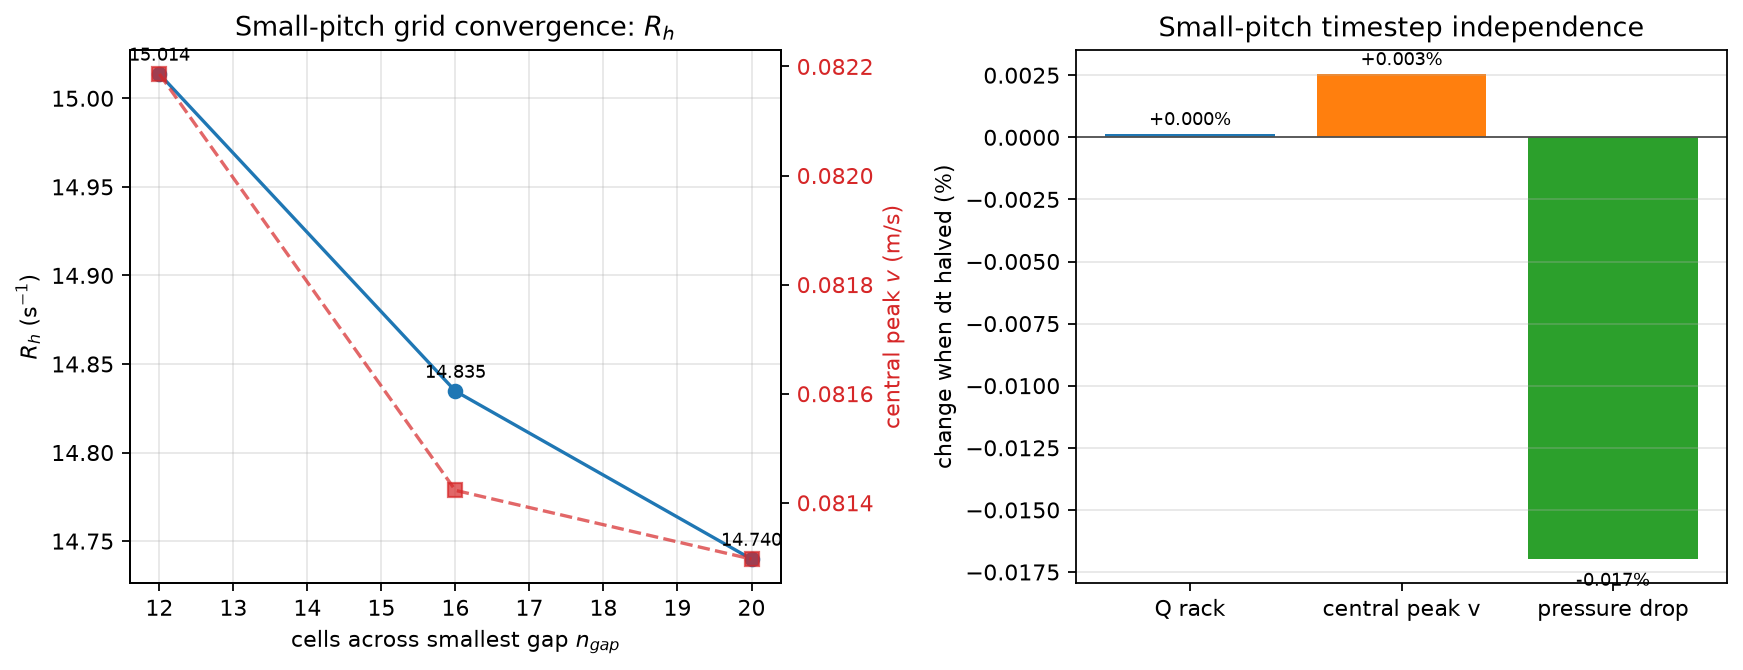
\includegraphics[width=0.95\textwidth]{grid_timestep_small}
\caption{Left: $R_h$ (blue) and central peak $v$ (red) versus mesh resolution,
converging with refinement. Right: relative change of observables when the
timestep is halved -- all below $0.02\%$.}
\end{figure}

\section{Flow fields}
\begin{figure}[H]
\centering
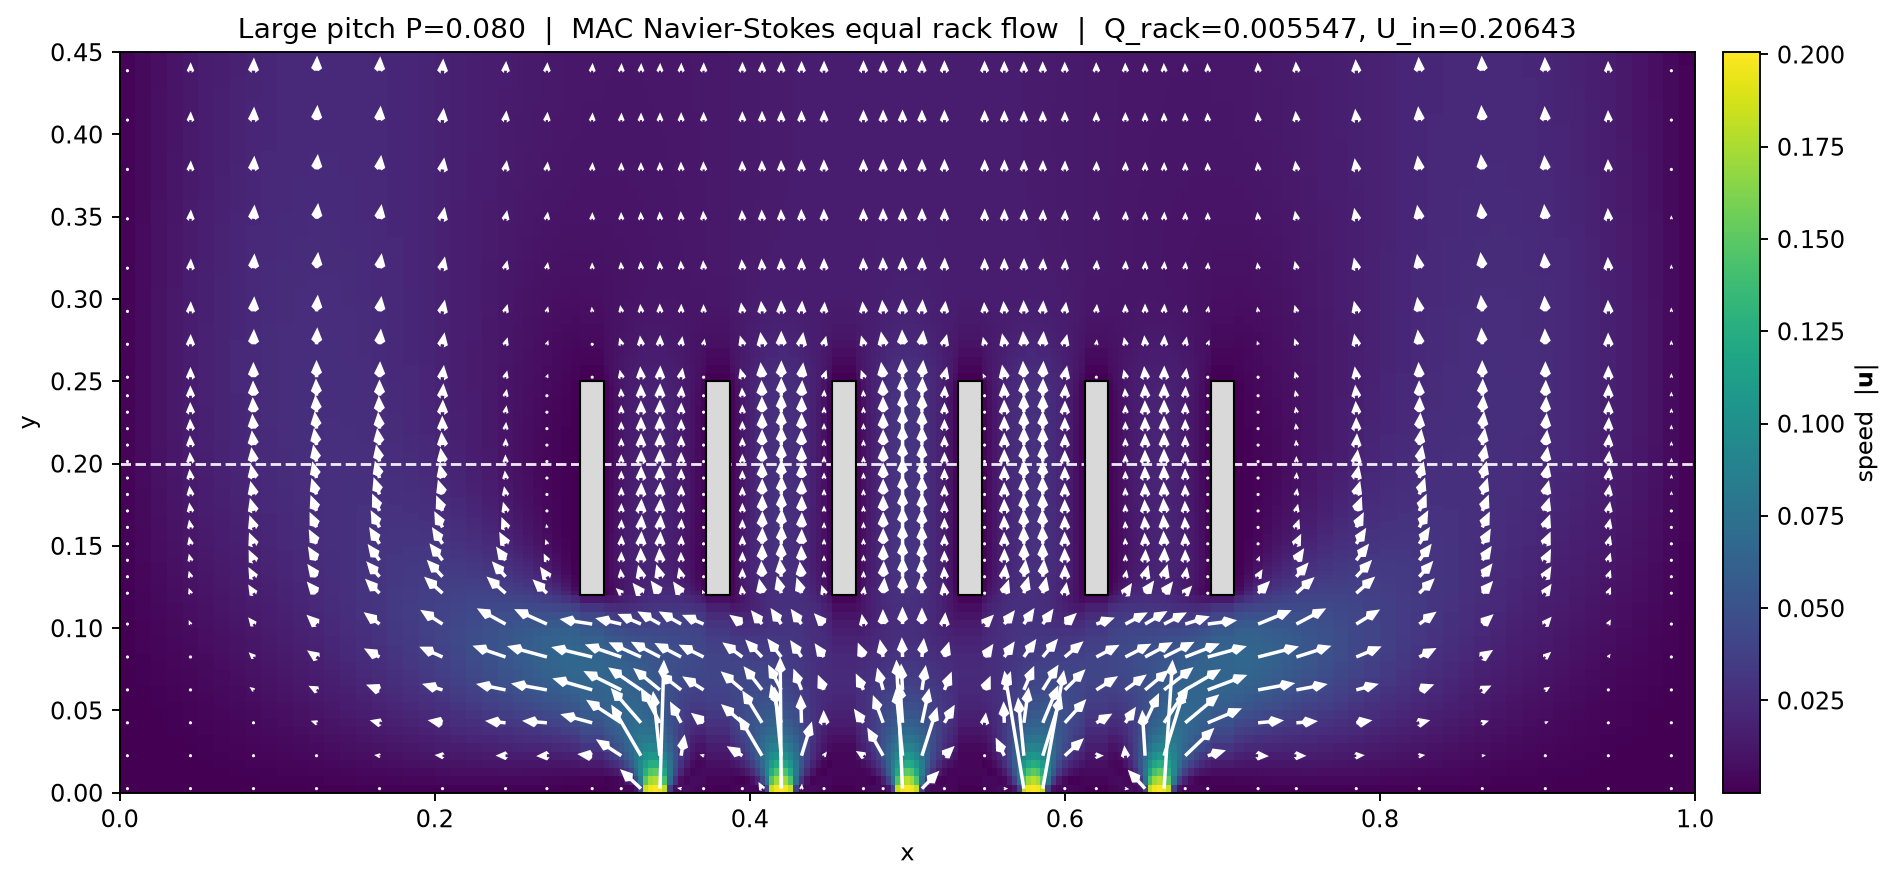
\includegraphics[width=0.93\textwidth]{field_large_2d}
\caption{Large-pitch ($P=0.080$) velocity vector field; colour is speed
$|\mathbf{u}|$, white arrows the velocity, gray blocks the wafers, dashed line
the $y_\mathrm{cut}=0.20$ flux line.}
\end{figure}

\begin{figure}[H]
\centering
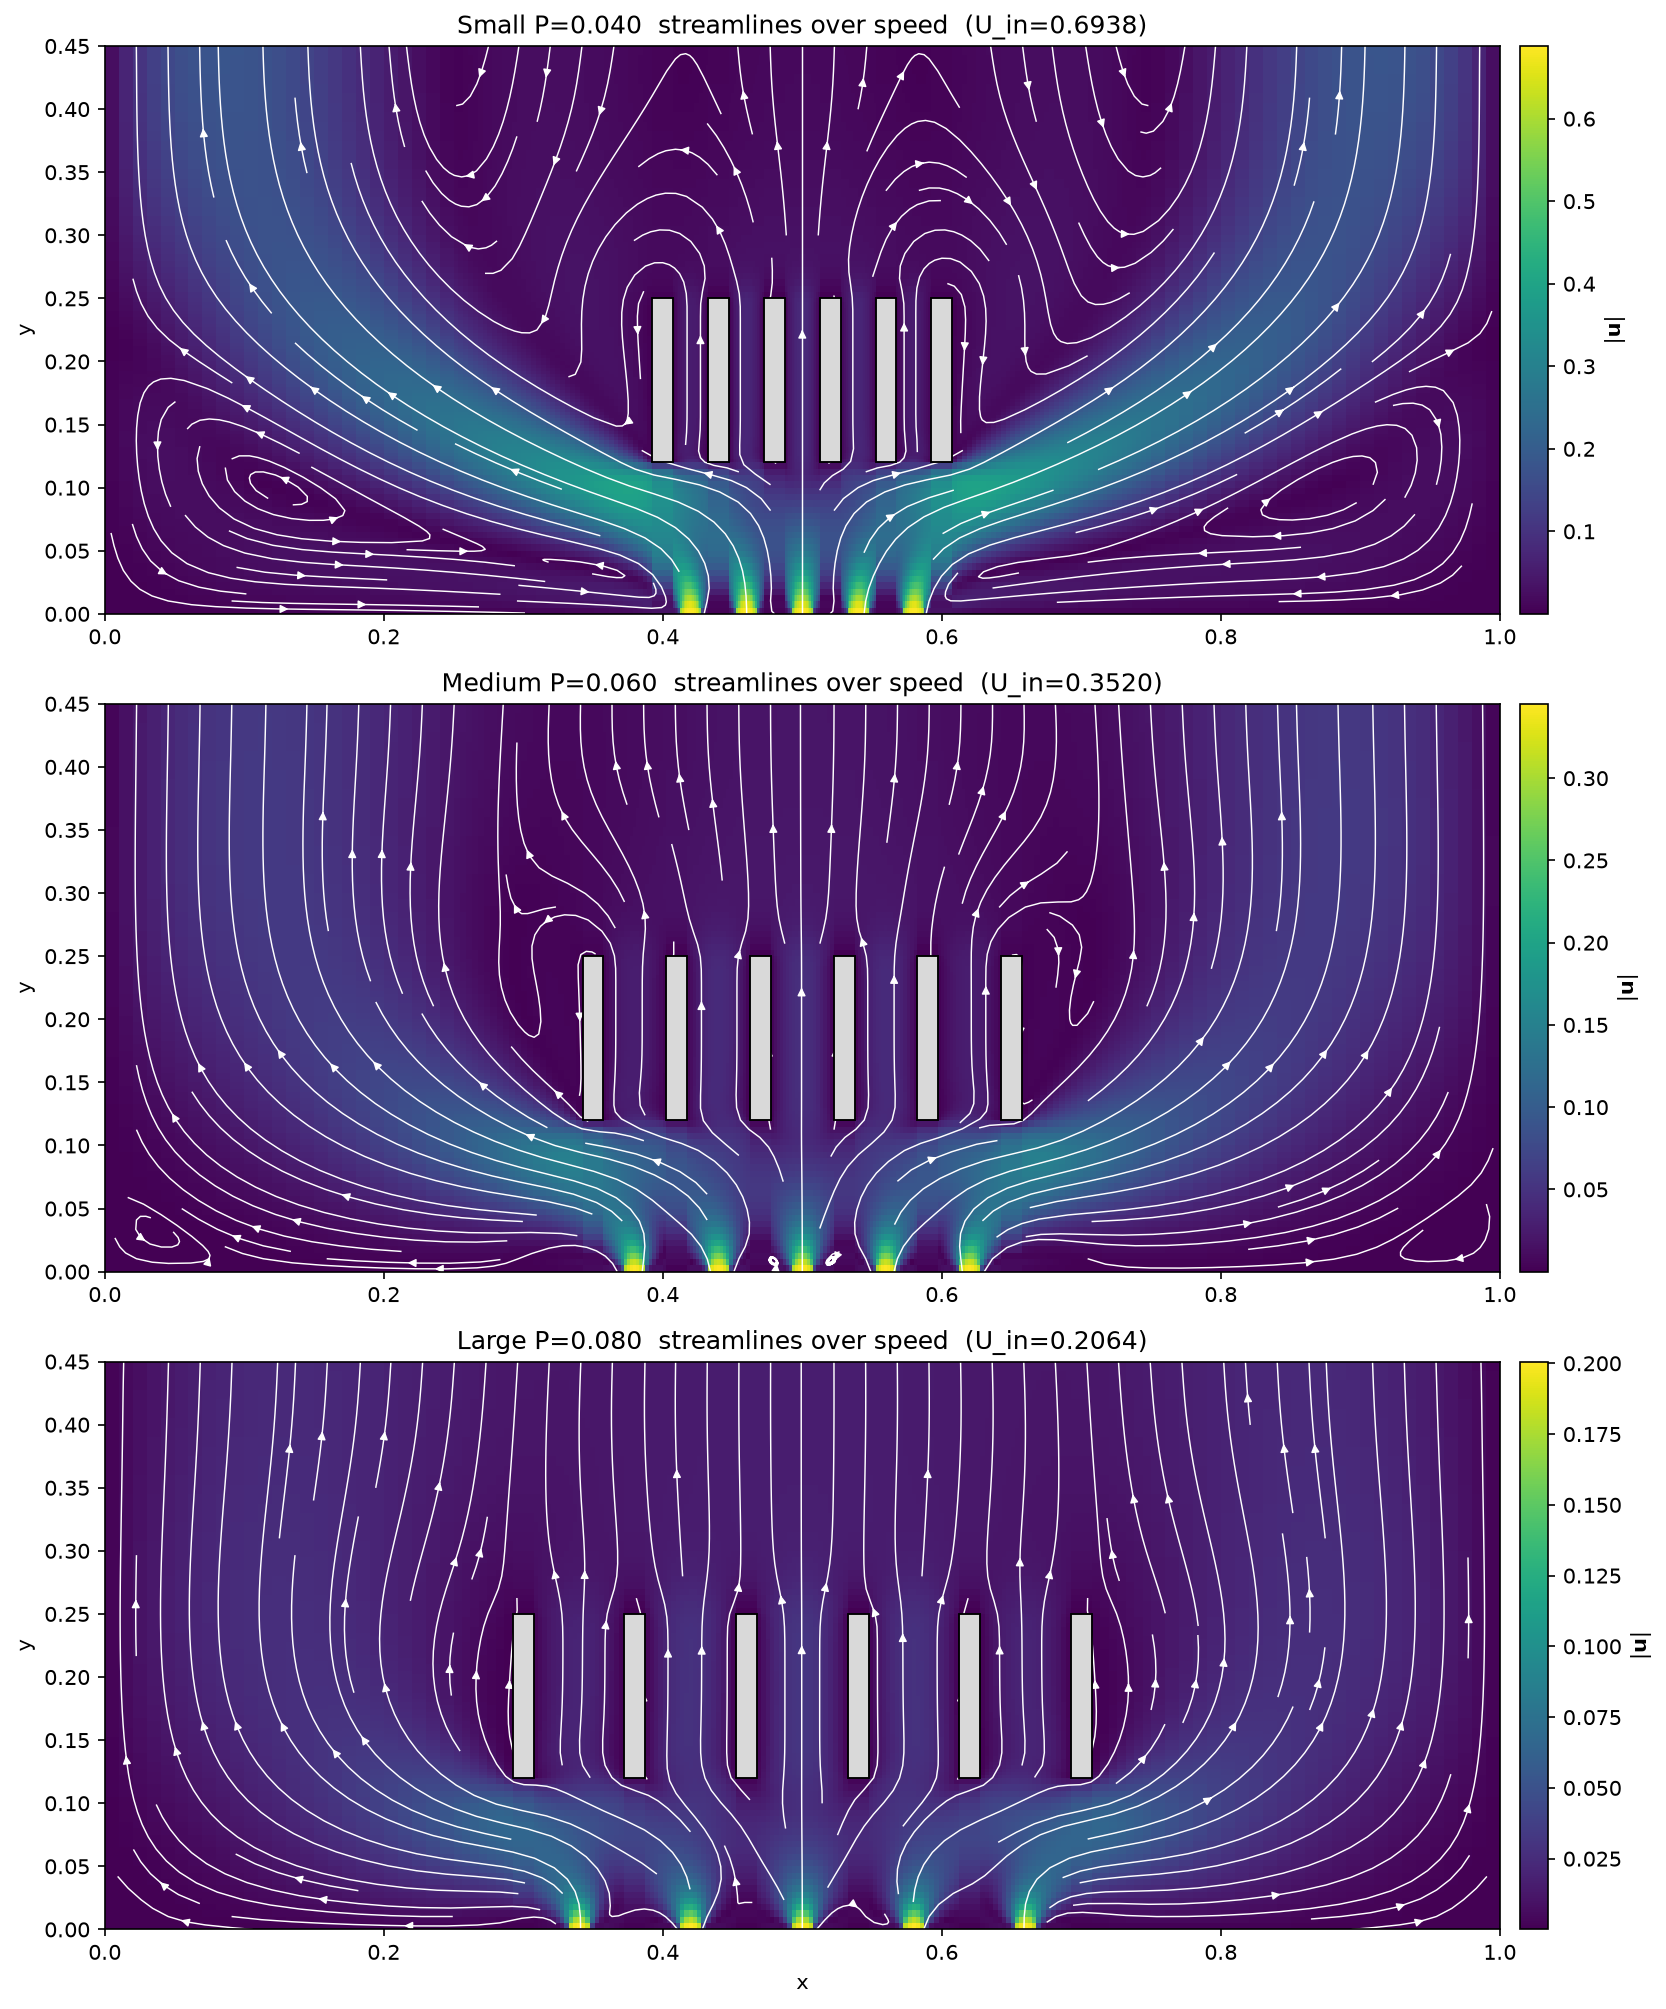
\includegraphics[width=0.93\textwidth]{streamlines_all}
\caption{Streamlines over speed for the three pitches (velocity interpolated to a
uniform grid for streamline tracing).}
\end{figure}

\begin{figure}[H]
\centering
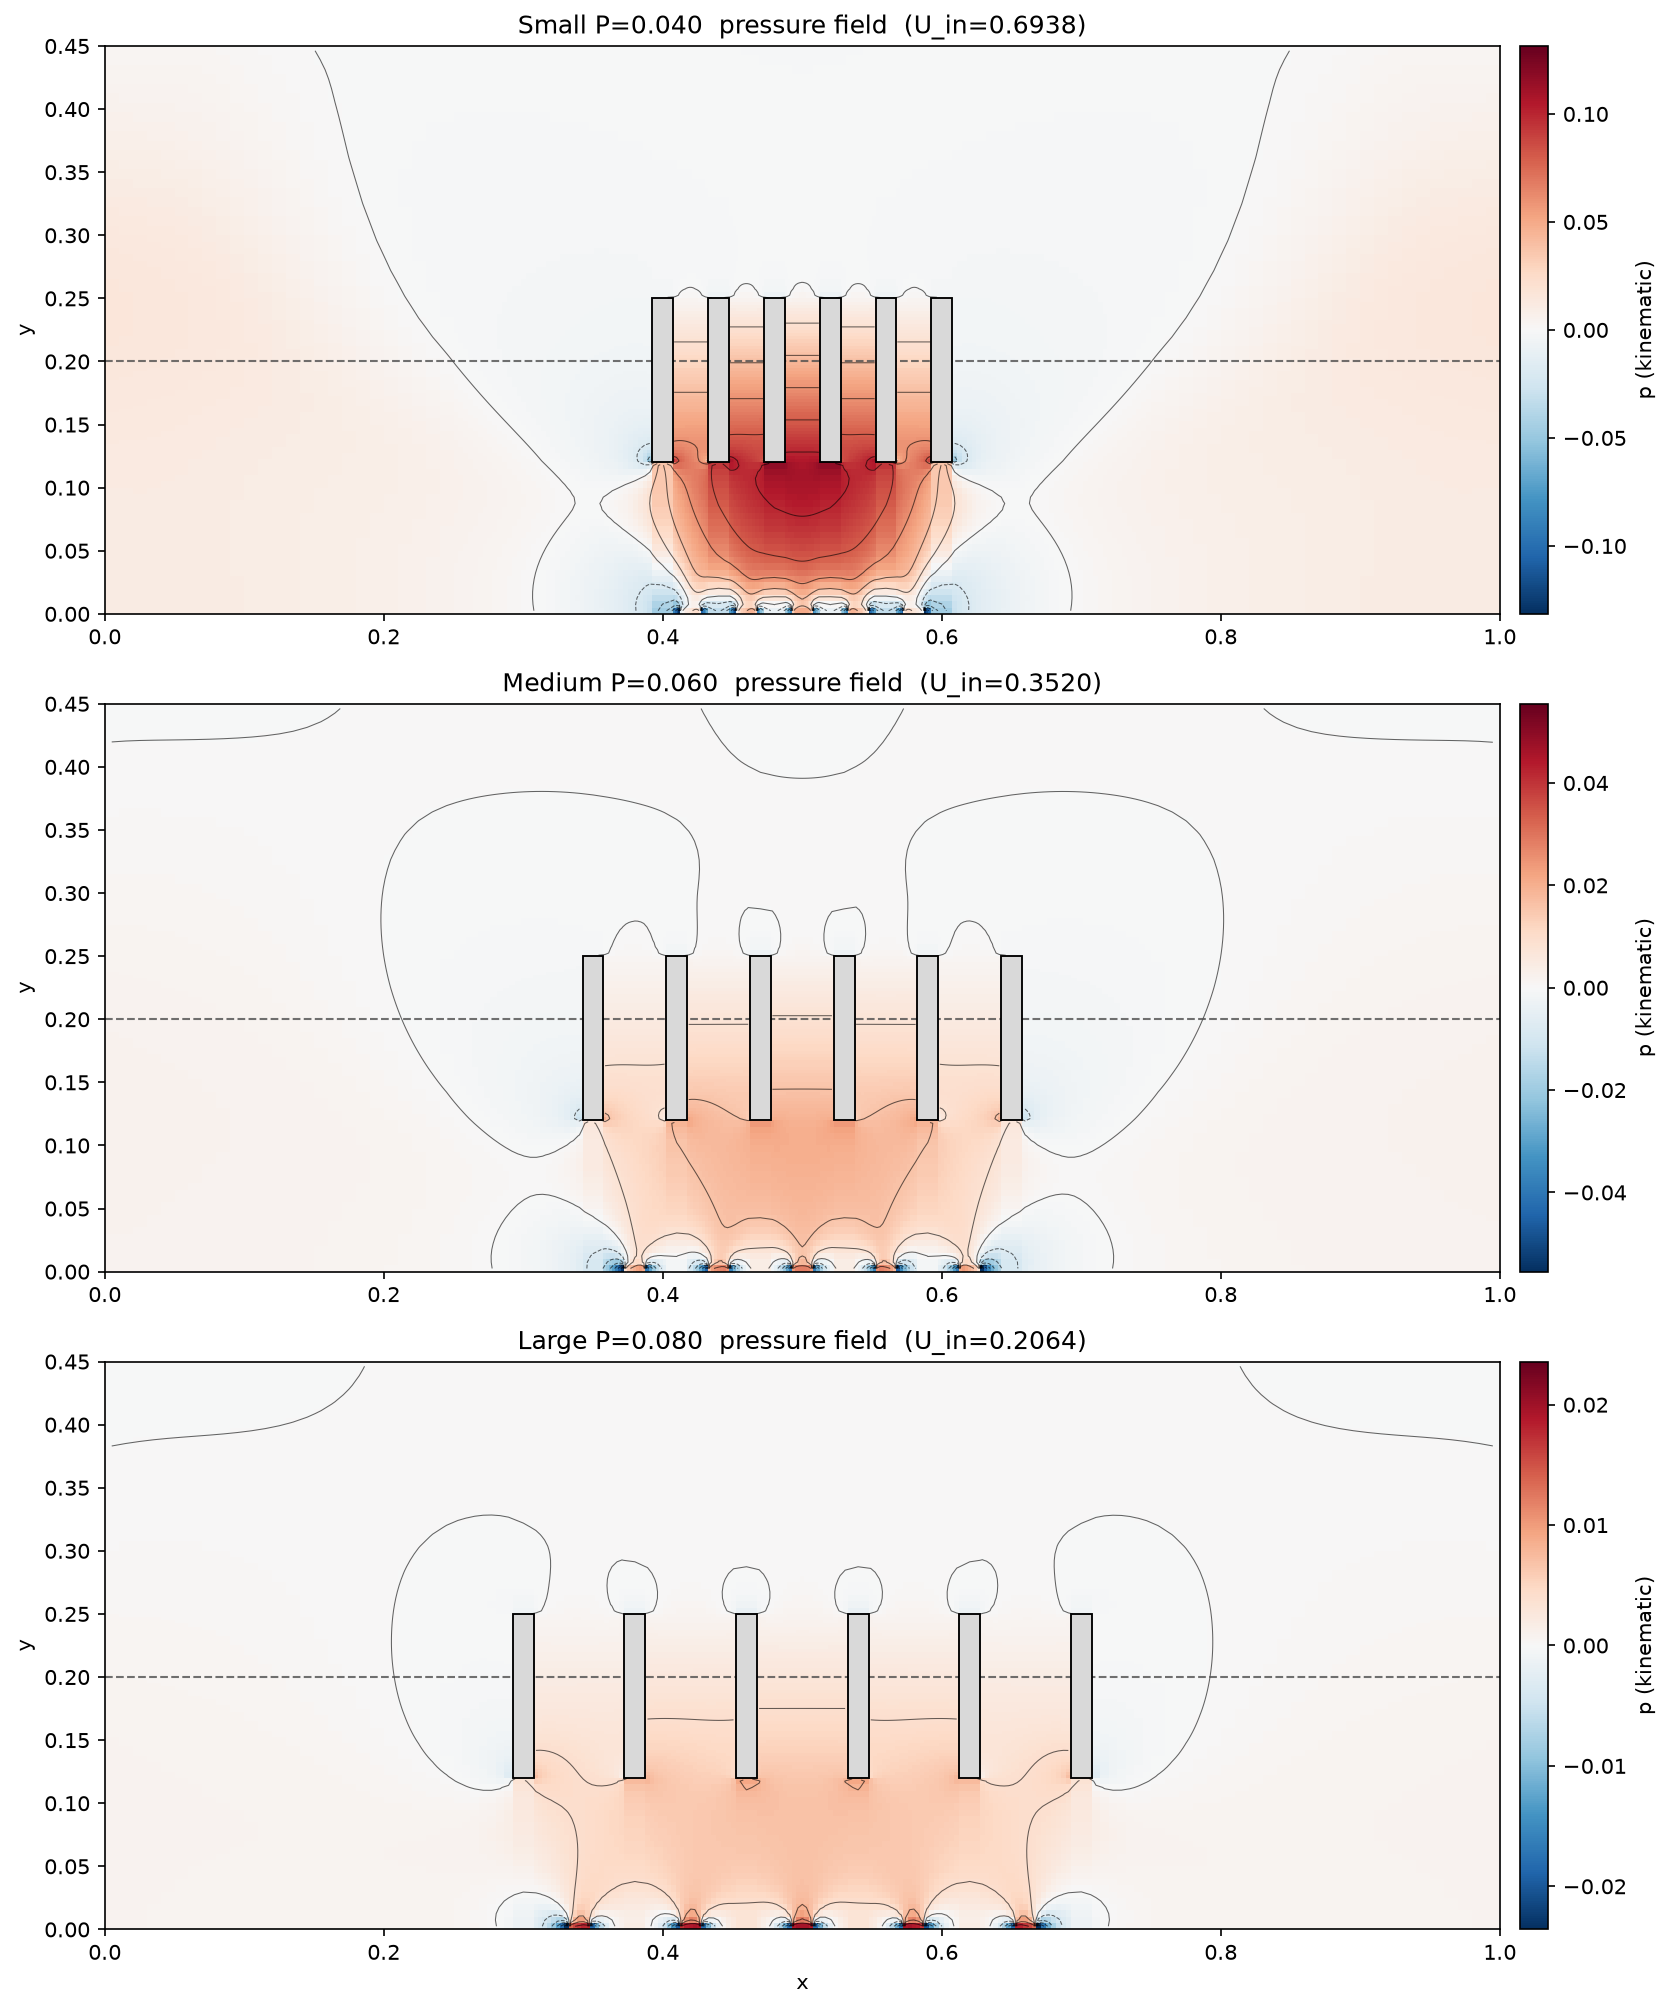
\includegraphics[width=0.93\textwidth]{pressure_all}
\caption{Kinematic pressure field with contours. Pressure drop across the rack
grows sharply as the pitch tightens, consistent with the $R_h$ ordering.}
\end{figure}

\section{Equal-$Q$ cut profiles}
\begin{figure}[H]
\centering
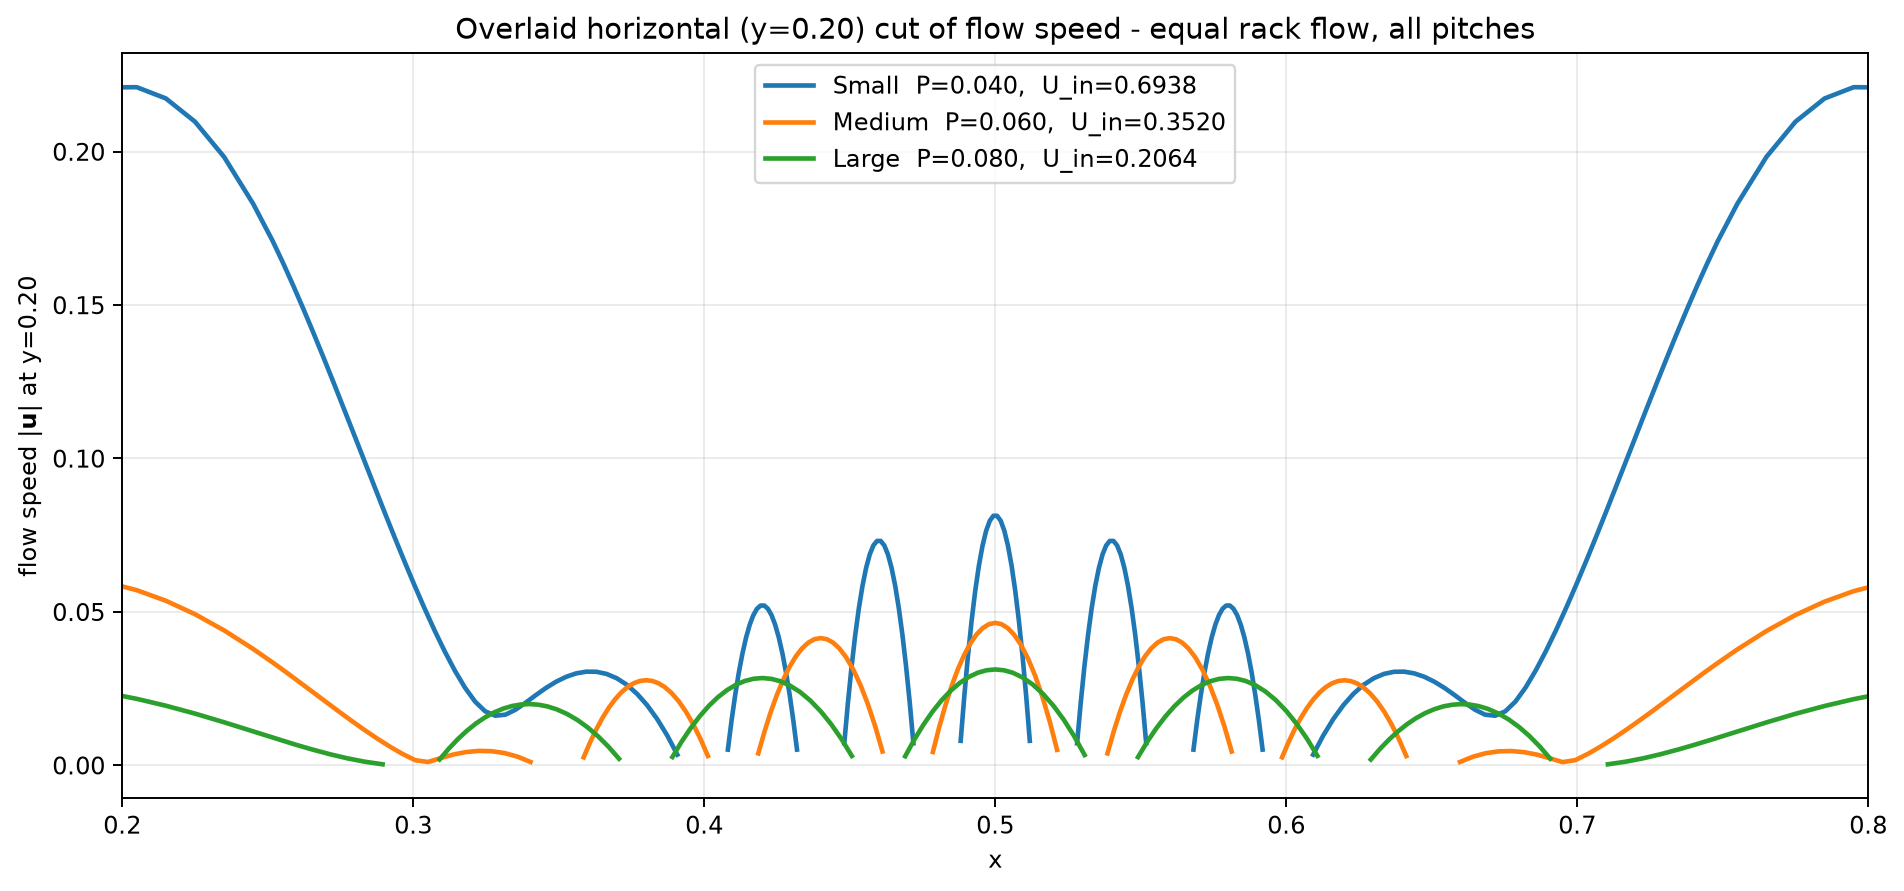
\includegraphics[width=0.80\textwidth]{ycut_speed_overlay}
\caption{Overlaid $y_\mathrm{cut}=0.20$ cut of flow speed. Tighter pitch reaches
a higher peak speed in the clear gaps to carry the common $Q_\mathrm{rack}$.}
\end{figure}

\begin{figure}[H]
\centering
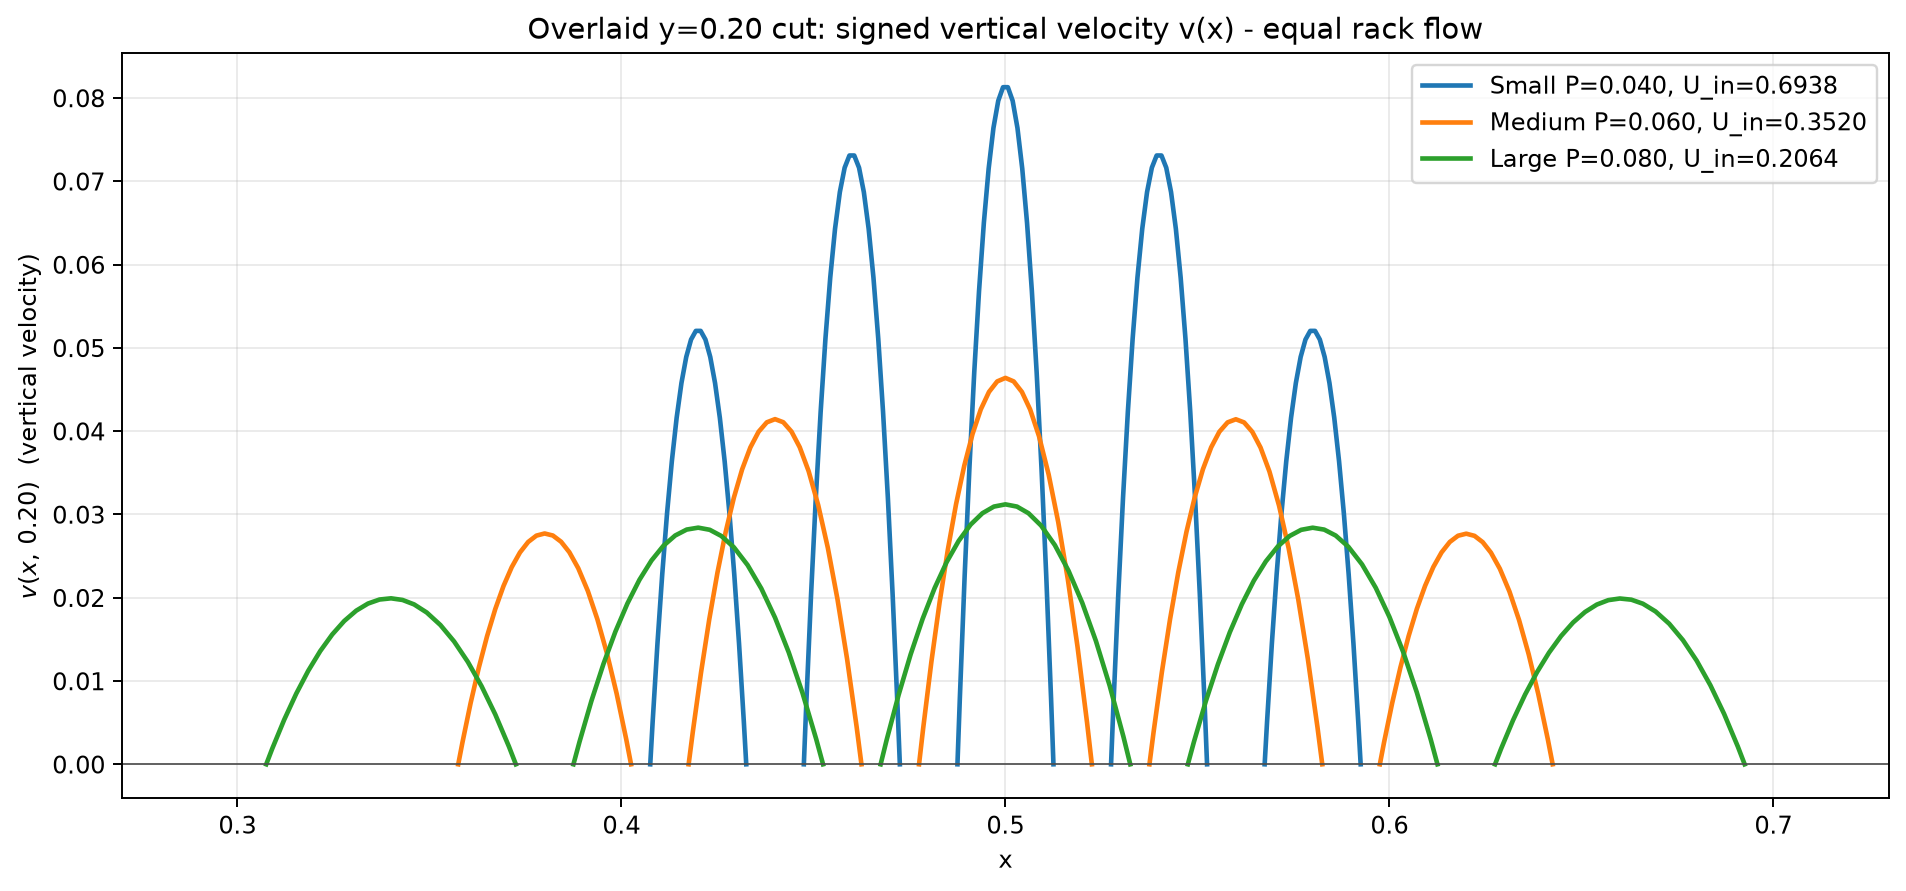
\includegraphics[width=0.80\textwidth]{ycut_v_overlay}
\caption{Overlaid $y_\mathrm{cut}=0.20$ cut of signed vertical velocity $v(x)$
over the five interior gaps (no-slip zeros imposed at wafer faces).}
\end{figure}

\section{Interpretation of the comparison}
The equal-$Q$ condition equalizes flow through the \emph{five interior gaps},
not the total inlet flow: a substantial and pitch-dependent fraction of the
inlet stream bypasses outside the rack span (visible as side flow in the field
plots), so only a minority of $Q_\mathrm{in}$ passes through the interior gaps,
and that minority fraction \emph{grows} with pitch. The result should therefore
be read as: the inlet speed is tuned per geometry to produce the same interior-gap
flow -- not as a comparison at equal pump flow or equal total inlet flow. On the
corrected (grid-aligned) geometry, the interior gaps carry only $10.7\%$ of the
inlet flow for Small, $21.0\%$ for Medium and $35.8\%$ for Large; the remainder
bypasses outside the rack span (visible as side flow in the field plots), and
the interior-gap share grows with pitch.

\section{Caveats and open validation items}\label{sec:caveats}
The following limitations bound how the quantitative results may be used:
\begin{itemize}\itemsep2pt
\item \textbf{Discrete inlet widths (corrected).} The inlet slot edges are now
exact $x$-grid faces, so every discrete slot is $0.0150\,$m and the total inlet
width is $0.0750\,$m for all pitches. This removed the earlier $10$--$13\%$
under-sizing and lowered $U_\mathrm{in}$ for Medium and Large accordingly.
\item \textbf{Approximate steady state.} See \S\ref{sec:conv}: acceptance is a
tightened, enforced steady-state gate (not an exact converged state).
\item \textbf{Pressure-tap sensitivity.} $R_h$ depends on the tap planes
(\S\ref{sec:taps}). On the corrected Large field, the default planes give
$R_h=0.987$; moving them just outside the wafer ends ($y=0.1175/0.2525$) gives
$1.070$ ($+8.4\%$) and farther out ($y=0.0775/0.2975$) gives $0.945$ ($-4.2\%$).
Only the ordering is tap-robust.
\item \textbf{Grid/timestep convergence (Small, demonstrated).} A three-mesh
refinement and a timestep halving were run for the Small case (\S\ref{sec:grid}):
timestep error is negligible ($<0.02\%$) and $R_h$ is monotone-converging with
$\sim\!0.6\%$ residual at the production mesh, so absolute $R_h$ is good to
$\sim\!1\%$ for Small. Medium and Large have not yet had the same refinement, so
their absolute values carry at least a comparable (unquantified) grid
uncertainty; the large separation between the three $R_h$ makes the ordering
robust regardless.
\item \textbf{Reproducibility, not independent verification.} The rerun harness
imports the production \texttt{Solver}; it checks reproducibility and cannot
expose an error shared by that implementation.
\end{itemize}

\section{Conclusions}
The MAC projection solver is discretely consistent and mass-conserving to
roundoff. The equal-$Q$ root solve reliably drives $Q_\mathrm{rack}$ to the
common target, and the corrected code gives hydraulic resistances
$R_h = 14.740 > 2.728 > 0.987$ (Small $>$ Medium $>$ Large) \emph{for the
present discretization}, essentially unchanged by the inlet correction. With the
inlet slots grid-aligned, the corrected inlet speeds are
$U_\mathrm{in}\approx 0.694/0.352/0.206$ (Small unchanged; Medium and Large lower
than the pre-alignment $0.388/0.237$, because the earlier slots were $10$--$13\%$
undersized). These remain reproduced computations, not yet mesh-independent,
physically validated quantities (\S\ref{sec:caveats}); a grid-refinement and
timestep study is the next step before the absolute $U_\mathrm{in}$, $\Delta p$
and $R_h$ can be called discretization-independent. The absolute speeds also
differ from the legacy finite-difference model's ($0.5605/0.3000/0.1833$)
because the numeric target $Q_0$ was carried over as a fixed constant rather than
redefined self-consistently for the MAC discretization.

\end{document}
